Para el plan de acción, no se tiene algo bien establecido, debido a que el plan de acción dependerá directamente del umbral que se esté excediendo. Es decir, el comportamiento será distinto si se excede el uso de memoria ram, a diferencia de que se exceda el uso de espacio en disco.
\newline
Lo que se realizó para el plan de acción fue únicamente detectar cuando ciertos recursos del dispositivo excedían los umbrales establecidos, y en caso de ser así, se envía un correo electrónico cada vez que alguno de los umbrales se excedía.
\newline
En la siguiente imagen se muestra el ejemplo para el uso del CPU, en el cual se utilizó el valor actual del uso de CPU devuelto con el comando SNMPGET, así como algunas banderas que nos permitían saber si se debía enviar el correo o no (para evitar enviar demasiadas veces un correo electrónico).

\pagebreak
\begin{figure}[htbp!]
	\centering
		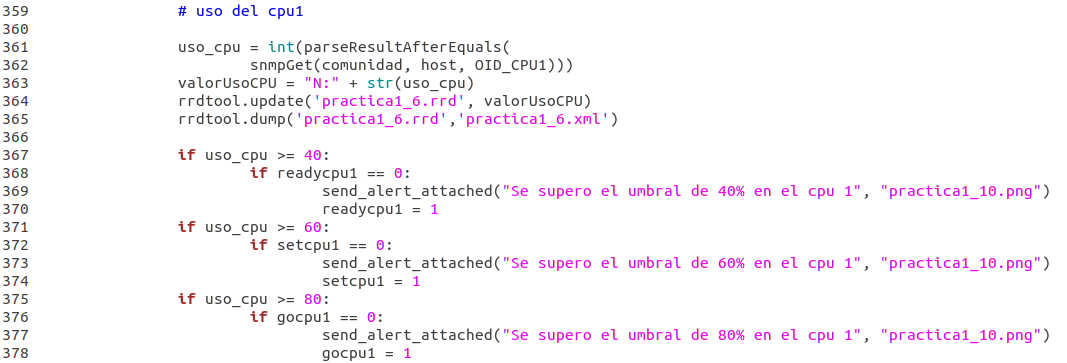
\includegraphics[width=0.8\textwidth]{imagenes/LineaBase/envioAlertaLineaBase.png}
	\caption{Uso de banderas para enviar el correo electrónico en caso de sobrepasar algún umbral.}
\end{figure}

También se hizo uso del protocolo SMTP para poder enviar los correos electrónicos, mediante el uso del servidor de Gmail. En el correo se pone como asunto qué umbral fue el que se superó, y de igual forma se adjunta la gráfica del monitoreo de dicho recurso hasta antes de que se superara el umbral.

\pagebreak
\begin{figure}[htbp!]
	\centering
		\includegraphics[width=0.8\textwidth]{imagenes/EnvioEmail.png}
	\caption{Uso del protocolo SMTP para enviar el correo electrónico.}
\end{figure}